\documentclass[a4paper]{article}
\usepackage{graphicx}
\usepackage{url}
\usepackage{wrapfig}

\begin{document}

\section{What's up with pbuilder?}

This is a document to explain what is pbuilder, what has been happening
recently with pbuilder, and what will probably happen in the near
future.

\subsection{Concepts of using pbuilder}

pbuilder facilitates clean-room environment testing of package building
through using a chroot image and extracting a fresh chroot image for
every build.

There are several simple commands for operation. \texttt{pbuilder
create}, \texttt{pbuilder update}, and \texttt{pbuilder
build}\footnote{pdebuild command is often more convenient} commands are
the typical commands used. If you need more details, see pbuilder
manual, \url{/usr/share/doc/pbuilder/pbuilder-doc.html}

When everything is set, \texttt{pbuilder build} will accept 
\texttt{.dsc} file (the Debian source-package) and build the package
inside the chroot.

\begin{tabular}{|l|l|l|}
\hline
operation & operation frequency & context \\
\hline
create & once per base.tgz & create the base filesystem \\
update & once per day (unstable update) & update the base filesystem \\
build & once per package & build the Debian package inside chroot \\
\hline
\end{tabular}

\newpage{}
\subsection{A developer use-case in using pbuilder}

Let me examine a typical sequence of events in a day of a Debian Developer.

%\begin{wrapfigure}{rt}{0.4\hsize}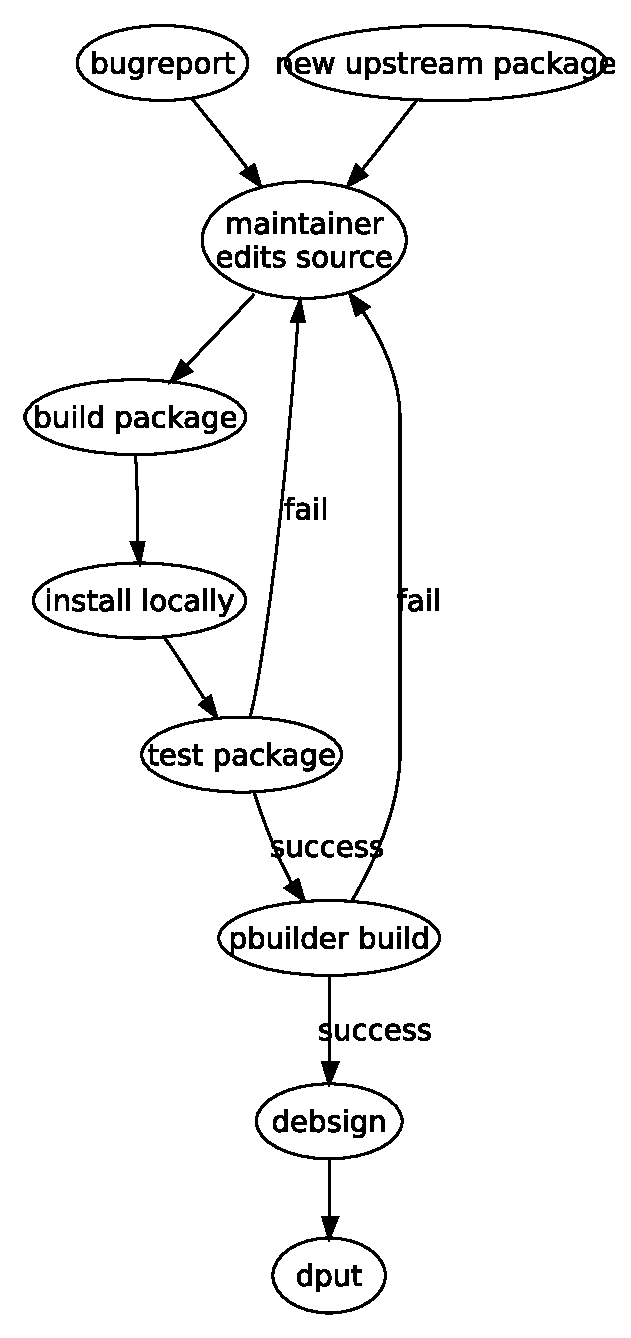
\includegraphics[width=1\hsize]{develcycle.eps}\end{wrapfigure}

\begin{center}
 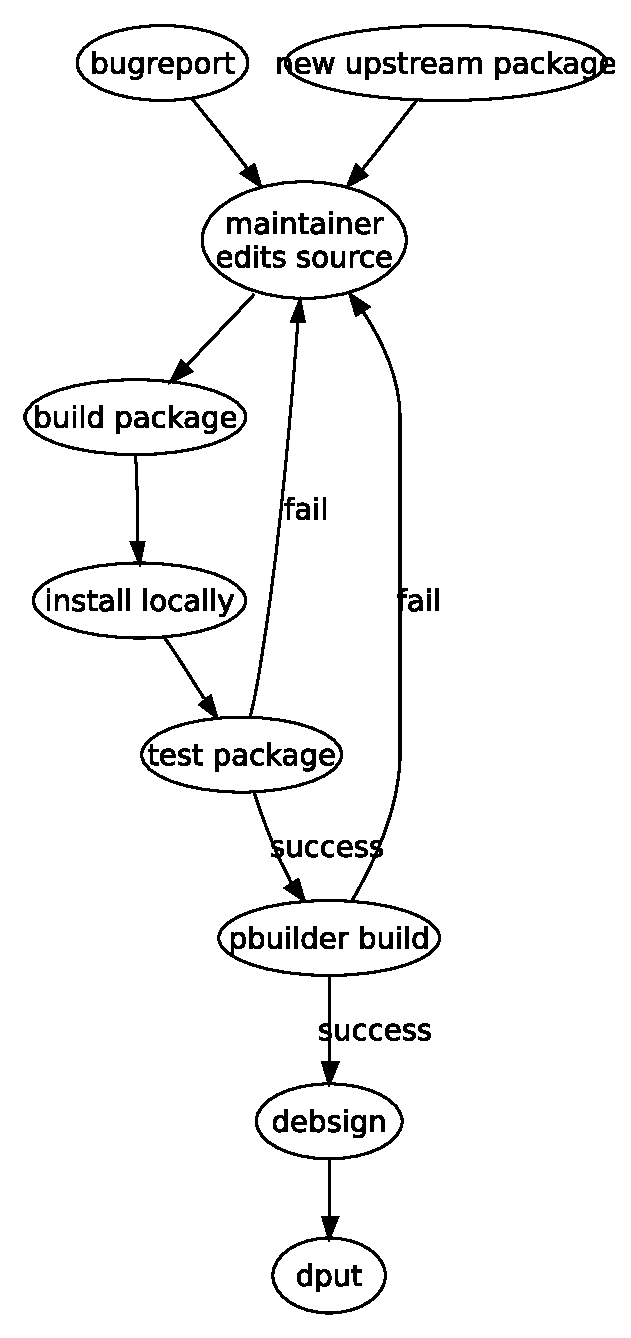
\includegraphics[width=0.6\hsize]{develcycle.eps}
\end{center}

pbuilder is built in to the process as a checking system to ensure
package quality.  \footnote{This is an example. Some people do not build
package locally and entirely work inside chroots.}

\subsection{Development structure}

Currently pbuilder is co-maintained with resources provided by Alioth.
Development is done mostly by Lo\"ic Minier and Junichi Uekawa.

Project page is available at 
\url{http://alioth.debian.org/projects/pbuilder}
and home page is available at, 
\url{http://pbuilder.alioth.debian.org/}
which provides the pbuilder manual.

git is used for source code management, and the repository can be
checked out by any of the following commands\footnote{ssh access
requires account on alioth}.

\begin{verbatim}
git-clone git://git.debian.org/git/pbuilder/pbuilder.git
git-clone http://git.debian.org/git/pbuilder/pbuilder.git
git-clone ssh://git.debian.org/git/pbuilder/pbuilder.git
\end{verbatim}

\subsection{Derivatives and their status}

\subsubsection{user-mode-linux port}

pbuilder-uml port exists. Apparently, it is working for most people.
Mattia Dongili has been working on this port.

base.tgz extraction is replaced with UML cow device support, and thus is
much faster.

\subsubsection{LVM port}

Someone did a port to using LVM snapshot for base-management.  There was
some mail posted, but noone really picked it up.

\subsubsection{cowdancer port}

Junichi Uekawa has been working on the port to cowdancer since 2005, and
it is somewhat stable.  This replaces base.tgz extraction with
\texttt{cp -la }, which is much faster.

Because of the way cowdancer hooks libc calls like open/close, it may
interfere with package building.  \footnote{etch release unfortunately
was faced with Bug 413912}

\subsubsection{qemu port}

Junichi Uekawa has been working on the port to qemu/kqemu/kvm since
early 2007. QEMU has COW block device support, so it eliminates the need
to extract base.tgz.

qemu port has an interesting advantage in that it adds
cross-architecture-building support for pbuilder. I can potentially
build and test ARM packages on my i386 box.

\subsection{Further development ideas}

\subsubsection{Installation testing}

There are other projects such as piuparts which can be leveraged by
pbuilder.  

pbuilder does provide example script for testing installation:
\url{/usr/share/doc/pbuilder/examples/execute_installtest.sh}.

\begin{verbatim}
pbuilder execute \
  /usr/share/doc/pbuilder/examples/execute_installtest.sh \
  pbuilder
\end{verbatim}

This command will try to install the package using apt-get into the
chroot.

\subsubsection{Package testing}

Package testing is a feature that is usually useful, especially since
developer time is limited, and repeated manual testing is no fun.
pbuilder includes an example hook script
\url{/usr/share/doc/pbuilder/examples/B92test-pkg} which will test
package after a successful build.

The test files are shell scripts placed in
\verb!debian/pbuilder-test/NN_name! (where NN is number) following
run-parts standard for file names \footnote{no '.' in file names!}.

\subsubsection{aptitude}

pbuilder exclusively depends on apt-get.  It might be time to look at
what is missing to get aptitude working.

\subsubsection{apt-key support}

pbuilder currently lacks apt-key support.  Since apt-key support is
definitely available in the current stable releases, it is about time to
start considering supporting apt-key.

\subsubsection{build-dependency}

Build-dependency parser has been somewhat old and suboptimal.  Lo\"ic
Minier has been working on refreshing it.

\subsubsection{buildd.net-like support}

pbuilder creates a bunch of useful build logs, but it lacks the
infrastructure to aggregate and put them to use.  Some projects to
create \texttt{pbuildd} did exist, but I am not sure if it still exists
today.

\subsection{References}

\begin{itemize}
 \item \url{http://pbuilder.alioth.debian.org/} or
 \url{/usr/share/doc/pbuilder/pbuilder-doc.html}: pbuilder manual
\end{itemize}

\end{document}
